%%
%% Dit is een subdocument van het projectplan.
%%
%% voorlopige indeling volgens SE Sommerville p623

\section{Planning}

\subsection{Introduction}
This project concerns building an expert tool called WickedXmas. To understand the problem very well, it requires a deep domain analysis . This excercise must start before any implementation can start so the first part of this project plan is a plan driven approach while for the construction an agile approach is chosen. 

\subsection{Organisation}
 %% hoe zijn wij als team geörganiseerd, wie zijn we en wat zijn onze rollen

\subsection{Risk analysis}
 %% wat zijn de mogelijke project risico's

\subsection{Hard- and software requirments}
 %% wat hebben we allemaal nodig om het ding te bouwen

\subsection{Work breakdown}

\begin{enumerate}
	\item \underline{\textbf{Startup}}
	\begin{itemize}
		\item Stakeholder meeting.
		\item Define the problem.
		\item Collect high-level requirments.
		\item Explore architectural solutions.
		\item Find tool and IDE options.
		\item Planning. 
	\end{itemize}
	\paragraph{Result}
	This block delivers a document that describes the problem , high-level requirements, business case ,risks , stakeholders, vision and challenges, technical options and a project plan.
	
	\item \underline{\textbf{Research}}
	\begin{itemize}
		\item Domain analysis.
		\item Context research.
		\item Find requirements based on using the current product tool.
		\item Find requirements based on sourcecode of the current product tool.
		\item Collect requirements.
		\item Stakeholder meeting.
	\end{itemize}
	\paragraph{Result}
	Domain research is added to the document, the result is a refined document with new requirements and choices with argumentation. Technical choices are made and the team has gained knowledge of IDE, tools and domain. 
	
	\item \underline{\textbf{Construction}}
	
	\begin{itemize}
		\item Iteration 1 :
		Create *xmas skeletons, GUI design and documentation
		\item Iteration 2 :
		Implement *xmas functionality, GUI and documentation
		\item Iteration 3 :
		Create *analysis/checkers skeletons, GUI design and documentation
		\item Iteration 4 :
		Implement *analysis/checkers functionality, GUI and documentation
		\item Iteration 5 :
		Implement additional options (Export,Report,...)
	\end{itemize}
	(*) xmas is the part that enables editing an xmas network, while analysis/checkers concerns the part that analyse and checks such a network.
	
	\paragraph{Result}
	Each iteration takes about 2 to 4 weeks and starts with an analysis , implementation , testing, documenting and a release (prototype). The aim of the last iteration is to deliver a fully working release of the product.
	
	\item \underline{\textbf{Final}}
	\begin{itemize}
		\item Product
		\item Documentation
		\item Presentation
	\end{itemize}
	\paragraph{Result}
	Product is ready and presented to the stakeholders.
\end{enumerate}

\subsection{Schedule}
 %% dit onderdeel moet vermoedelijk in het schedule plan
  

  \begin{figure}
  	\centering
  	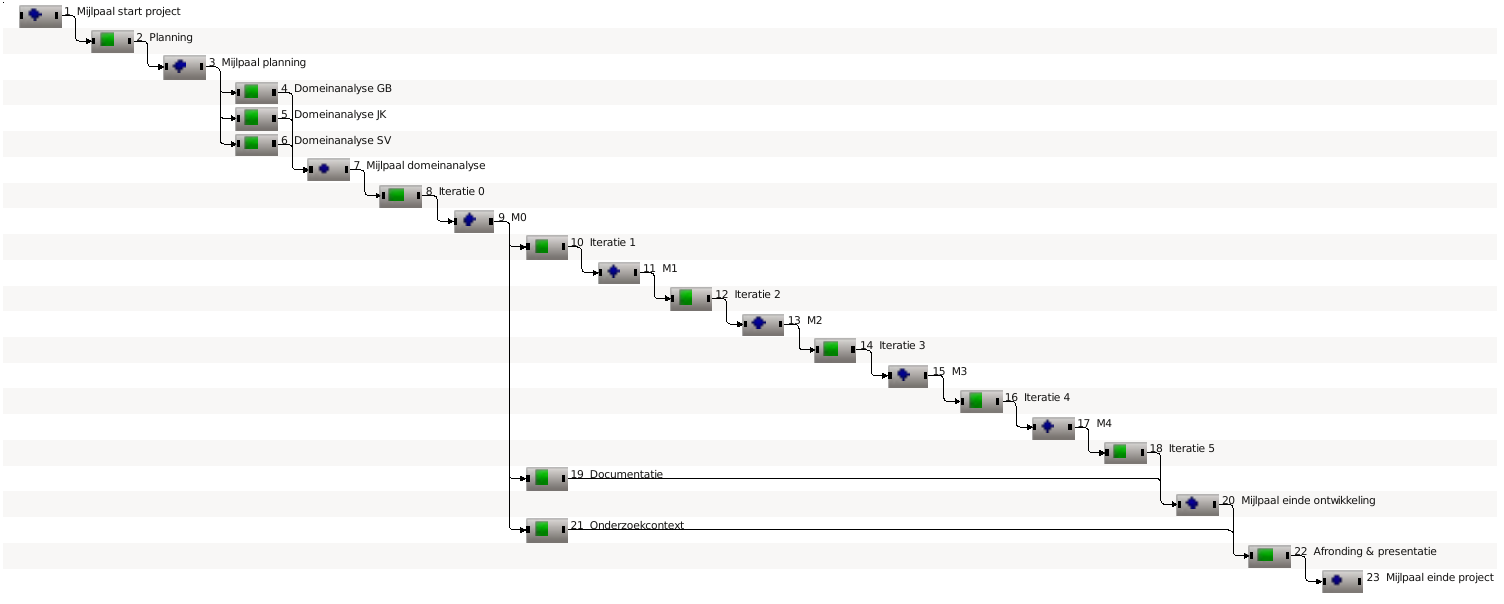
\includegraphics[width=0.8\textwidth,natwidth=1306,natheight=543]{Gantt.png}
  	\caption{\label{fig:Gantt Chart}Scheduling.}
  \end{figure}

\begin{tabular}{ll}\hline
{\bf Fase}    & {\bf weken}\\\hline
Planning             & 2,5 \\

Domeinanalyse        & 3 \\
Architectuur         & 3 \\

Iteratie 1           & 3 \\
Iteratie 2           & 3 \\
Iteratie 3           & 3 \\
Iteratie 4           & 3 \\
Iteratie 5           & 3 \\

Onderzoekcontext     &	2 \\

Afronding	     & 1.5 \\
\hline
Totaal               & 27 \\
\end{tabular}



\begin{itemize}
 \item 27 weken * 15 uur/week = 405 uur
 \item 8 maanden, ongeveer 32 weken beschikbaar, dus 5 weken marge
\end{itemize}



\paragraph{Capaciteitsplanning}

\begin{enumerate}
 \item vakanties?
 \item beschikbaarheid Freek en Bernard?
\end{enumerate}

\paragraph{Planning iteraties}
\begin{enumerate}
 \item 3 weken per interatie
 \item hoeveel tijd voor requirements?
 \item hoeveel tijd voor evaluatie?
\end{enumerate}






\subsection{Monitoring and reporting}
 %% hoe gaan we onze doelstellingen bewaken en rapporteren